% \section{Hilft Musik beim lernen?}
% Dieser Frage wollen wir im Folgenden auf den Grund gehen - beziehungsweise versuchen wir es. Ist das überhaupt möglich, die Frage zu beantworten?\\
% Dafür machen wir - was auch sonst - ein kleines Experiment! \\

% Überlege dir eine naturwisenschaftlich sinnvollle (das haben wir ja die letzten Stunden gelernt) Methode, wie man diese Frage beantworten kann.
% Dabei geht es noch nicht darum, dass das Experiment perfekt ist, es geht erst einmal nur darum, dass wir ein paar Ideen sammeln. Notiere dir aber,
% worauf man achten sollte, und welche Probleme es geben könnte. \\


% \writeLines{10}{\textwidth}

\newpage

    \subsection*{Aufgaben mit Musik}
        \subsubsection*{Aufgabe 1}
        Schreibe einen kleinen (zusammenhämgenden!) Fließtext darüber, was Naturwissenschaft ist, wofür wir sie brauchen
        und was man beim wissenschaftlichen Arbeiten  beachten sollte.

    \subsubsection*{Aufgabe 2}
        Berechne folgende Aufgaben im Kopf:

        \begin{align*}
            \randInt{10}{57}+48 & = \\
            455-\randInt{157}{399} & = \\
            3 \cdot \randInt{8}{17} +2 & = \\
            3 \cdot \randInt{21}{48} & = \\
            266 : 14 & = \\
        \end{align*}

    \subsubsection*{Aufgabe 3}
        Löse die folgende Textaufgabe:
        \begin{itemize}
            \item[] Louisa schoss in der letzten Saison doppelt so viele Tore wie ihr Mitspieler Tuncay. Julius erzielt 5 Tore weniger als Louisa.
                      Zusammen haben die drei 25 Tore geschossen. Wie viele Tore hat jeder Spieler erzielt?
        \end{itemize}

    \newpage
    \subsubsection*{Aufgabe 4}

        \begin{itemize}
            \item[a)] Vereinfache den folgenden Term:

                \begin{align*}
                & 8(5y-1)-40(y+1)-4+2y
                \end{align*}

            \item[b)] Löse die folgende Gleichung nach $x$ auf.
                \begin{align*}
                & 6x-5=25
                \end{align*}
        \end{itemize}



    % Gegeben sind folgende Messdaten, zusammen mit einer Ausgleichsgeraden: \\

    % \begin{minipage}{0.49 \textwidth}
    %     \begin{tikzpicture}[>=stealth]
    %         %grid
    %         \draw[help lines, color=gray!30] (0,0) grid (5,5);

    %         \draw[->](0,0)--(5,0) node[right]{$t$ [s]};
    %         \draw[->](0,0)--(0,5) node[left]{$s$ [m]};

    %         \foreach \x in {1,2,3,4}{
    %             \draw (\x,0.1)--(\x,-0.1) node[below]{$\x$};
    %             \draw (0.1,\x)--(-0.1,\x) node[left]{$\x0$};
    %         }

    %         %Messdaten
    %         \fill[orange](1,1.1)circle(0.1);
    %         \fill[orange](1.5,2.5)circle(0.1);
    %         \fill[orange](2,3.1)circle(0.1);
    %         \fill[orange](2.5,3.8)circle(0.1);
    %         \fill[orange](3,4.2)circle(0.1);



    %         \draw[dblue, thick](0,0)--(2,3)--(8/3,4);
    %     \end{tikzpicture}
    % \end{minipage}
    % \begin{minipage}{0.49 \textwidth}
    %     \begin{itemize}
    %         \item[a)] Stelle die Geradengleichung der Ausgleichgeraden auf.
    %         \item[b)] Welche Geschwindigkeit hat der Läufer?
    %         \item[c)] Wie lange benötigt er für 45m?
    %         \item[d)] Wie weit kommt er in 27s?
    %     \end{itemize}
    % \end{minipage}

    \subsubsection*{Aufgabe 4}
    Anna, Eva und Tina wohnen nebeneinander in drei Reihenhäusern. Sie spielen drei unterschiedliche Instrumente
    und betreiben drei unterschiedliche Sportarten.
    Folgende Informationen sind bekannt:\\

    \begin{itemize}
        \item[1.] Tina macht Judo.
        \item[2.] Das Mädchen im Haus ganz links spielt Klavier.
        \item[3.] Die Gitarristin spielt auch Badminton.
        \item[4.] Anna wohnt links von Tina.
        \item[5.] Eva wohnt direkt neben der Handballerin.
    \end{itemize}

    Wer spielt Flöte?

    \newpage

\subsection*{Aufgaben ohne Musik}
    \subsubsection*{Aufgabe 1}
        Beschreibe in einem kleinen Aufsatz, wie man wissenschaftlich überprüfen könnte,
        ob ein Objekt, welches man fallen lässt, zur gleichen Zeit den Boden erreicht, wie ein anderes Objekt, welches man zur gleichen Zeit nach vorne wirft.

    \subsubsection*{Aufgabe 2}
        Berechne folgende Aufgaben im Kopf:

        \begin{align*}
            \randInt{66}{98}+\randInt{22}{45} & = \\
            714-\randInt{218}{613} & = \\
            8/2-5 & = \\
            4 \cdot \randInt{26}{39} & = \\
            216 : 18 & = \\
        \end{align*}

    \subsubsection*{Aufgabe 3}
        Löse die folgende Textaufgabe:
        \begin{itemize}
            \item[] Bei einem Rechteck ist die Breite $8$ cm kürzer als die Länge. Der Umfang beträft 144 cm.
                    Berechne den Flächeninhalt des Rechtecks.
        \end{itemize}

    \subsubsection*{Aufgabe 4}

    \begin{minipage}[l]{0.6\textwidth}
        Stelle einen Term auf, um den Umfang der nebenstehenden Form zu berechnen.
    \end{minipage}
    \begin{minipage}[r]{0.35\textwidth}
        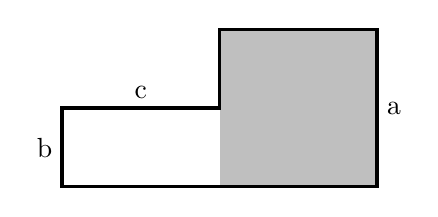
\begin{tikzpicture}
            \fill[lightgray](2,0) rectangle(4,2);
            \draw[very thick](0,0)--(0,1)--(2,1)--(2,2)--(4,2)--(4,0)--cycle;

            \node[right] at (4,1){a};
            \node[left] at (0,0.5){b};
            \node[above] at (1,1){c};
        \end{tikzpicture}
    \end{minipage}
        % Gegeben sind die folgenden Messdaten:

        % \begin{minipage}{0.49 \textwidth}
        %     \begin{table}[H]
        %         \centering
        %         \begin{tabular}{c|c}  % Spaltenformat: 'c' = zentriert, '|' = vertikale Linie
        %             \hline  % Horizontale Linie oben
        %             $t$ [s] & $v$ [m/s] \\  % Spaltenüberschriften mit mathematischen Variablen
        %             \hline
        %             0 & 0 \\
        %             1 & 2,1 \\  % Dezimalpunkt statt Komma in LaTeX
        %             2 & 3,9 \\
        %             3 & 6,0 \\
        %             4 & 8,2 \\
        %             \hline  % Horizontale Linie unten
        %         \end{tabular}
        %         \caption{Messwerte der Funktion}  % Beschreibung der Tabelle
        %         \label{tab:messwerte}  % Label für Referenzen
        %     \end{table}
        % \end{minipage}
        % \begin{minipage}[c]{0.49 \textwidth}
        %     \begin{itemize}
        %         \item[a)] Stelle die Tabelle graphisch dar.
        %         \item[b)] Stelle eine Funktionsgleichung der Ausgleichsgerade auf.
        %         \item[c)] Welche Geschwindigkeit hat das Objekt nach 8 s?
        %     \end{itemize}
        % \end{minipage}

        \subsubsection*{Aufgabe 4}
        Ernst, Moritz, Felix und Sebastian sind Brüder. Sie haben insgesamt 170 Tafeln
    Schokolade. Beim Verteilen bekommt Moritz eine Tafel mehr als Ernst, Felix bekommt 2
    Tafeln mehr als Moritz und Sebastian erhält 3 Tafeln mehr als Felix. Wie viele Tafeln
    Schokolade erhält Moritz?







% \subsection{Worum ging es?}
% Um etwas in die Welt der Naturwissenschaft einzutauchen haben wir in den
% letzten Stunden einige kleine Experimente durchgeführt, und zum Teil auch vollständig ausgewertet und diskutiert.\\
% Notiere dir hier, was wir in unseren Experimenten, die wir gemacht haben, rausfinden wollten. \\

% \writeLines{8}{\textwidth}

% \newpage

% \subsection{Wie sah das Experiment aus?}

% Beschreibe hier, was wir für ei Experiment gemacht haben, um herauszufinden, was wir rausfinden wollten.\\
% Warum war das geeignet? Du kannst gerne Skizzen benutzen (das ist sowieso immer sinnvoll ;-) \\

% \karoBox{\textwidth}{10cm}

% \newpage

% \subsection{Auswertung des Experimentes}

% Beschreibe nun, wie wir nun durch das Experiment unsere Anfangsfrage beantworten konnten.\\

% \karoBox{\textwidth}{9cm}

% \subsection{Was ist Naturwissenschaft?}

% Kannst du nun nocheinmal für dich auschreiben/definieren, was Naturwissenschaft ist, und wodurch sie sich auszeichnet? \\

% \drawbox{\textwidth}{3cm}